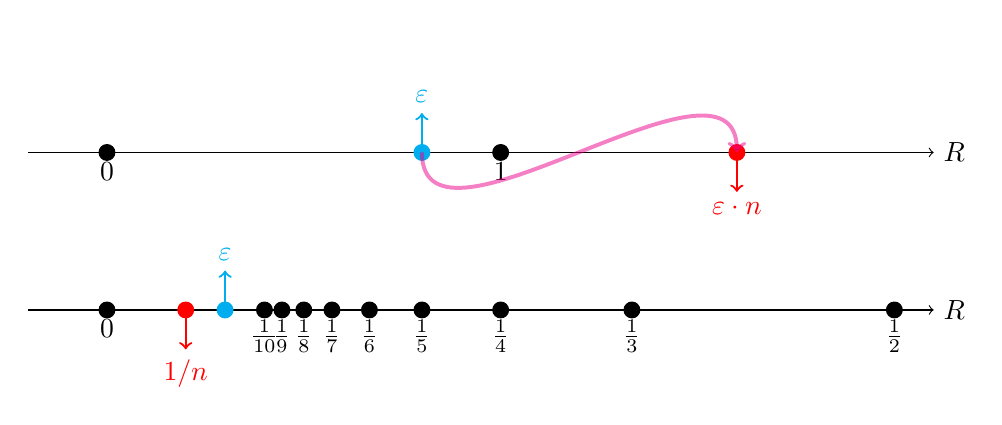
\begin{tikzpicture}[scale=2]
	\begin{scope}[yshift=1cm]
		\draw[->] (-0.5, 0) -- (5.25, 0) node[right] {$\mathbb{R}$};
		\filldraw[cyan] (2, 0) circle (0.05);
		\filldraw[red] (4, 0) circle (0.05);
		\filldraw[black] (2.5, 0) circle (0.05) node[anchor=north] {$1$};
		\filldraw[black] (0, 0) circle (0.05) node[anchor=north] {$0$};
		
		\draw[->, color=cyan, thick] (2,0) -- ++(0, +0.25) node[anchor=south] {\( \varepsilon \)};
		\draw[->, color=red, thick] (4,0) -- ++(0, -0.25) node[anchor=north] {\( \varepsilon\cdot n \)};
		
		\draw[->, color=magenta, line width=.5mm, in=90, out=-90, opacity=.5] (2,0) to (4,0);
	\end{scope}
	\draw[->] (-0.5, 0) -- (5.25, 0) node[right] {$\mathbb{R}$};
	\filldraw[cyan] (.75, 0) circle (0.05);
	\filldraw[red] (.5, 0) circle (0.05);
	\filldraw[black] (0, 0) circle (0.05) node[anchor=north] {$0$};
	
	% Set a value for epsilon on the number line
%	\pgfmathsetmacro{\eps}{0} % Position of epsilon
	
	% Define points for 1/n using calculations
	\foreach \n in {2, 3, ..., 10} {
		\pgfmathsetmacro{\pos}{10 / \n} % Scale positions for 1/n
		\draw[fill=black] (\pos, 0) circle (0.05) node[below] {$\frac{1}{\n}$};
	}

	\draw[->, color=cyan, thick] (.75,0) -- ++(0, +0.25) node[anchor=south] {\( \varepsilon \)};
	\draw[->, color=red, thick] (.5,0) -- ++(0, -0.25) node[anchor=north] {\( 1/n \)};	
		
%	\draw[decorate, decoration={brace, amplitude=10pt}, thick, color=green!75!black, opacity=.5] (5, -0.1) -- (10 / 3, -0.1) 
%	node[midway, below=10pt, color=green!80!black] {\( 1/6 \)};	
%	\draw[decorate, decoration={brace, amplitude=10pt}, thick, color=green!75!black, opacity=.5] (10/3, -0.1) -- (10/4, -0.1) 
%	node[midway, below=10pt, color=green!80!black] {\( 1/12 \)};
%	\draw[decorate, decoration={brace, amplitude=10pt}, thick, color=green!75!black, opacity=.5] (10/4, -0.1) -- (10/5, -0.1) 
%	node[midway, below=10pt, color=green!80!black] {\( 1/20 \)};	
\end{tikzpicture}

%\begin{tikzpicture}
%	% Draw the number line
%	\draw[->] (-0.5, 0) -- (8, 0) node[right] {$\mathbb{R}$};
%	
%	% Set a value for epsilon and scale positions for n * epsilon
%	\pgfmathsetmacro{\eps}{1} % Value of epsilon
%	
%	% Mark the value 1 on the number line
%%	\draw[fill=black] (1, 0) circle (0.05) node[above] {$1$};
%	
%	% Define points for n * epsilon using calculations
%	\foreach \n in {1, 2, 3, 4, 5, 6, 7} {
%		\pgfmathsetmacro{\pos}{\n * \eps} % Calculate position for n * epsilon
%		\draw[fill=black] (\pos, 0) circle (0.05) node[below] {$\n \cdot \varepsilon$};
%	}
%	
%	% Draw inequality arrow from 1 to the appropriate n*epsilon where 1 < n * epsilon
%%	\pgfmathsetmacro{\npos}{3 * \eps} % Position where 1 < n * epsilon (e.g., 3 * epsilon)
%%	\draw[thick, ->] (1.1, 0.3) -- (\npos - 0.1, 0.3) node[midway, above] {$1 < n \cdot \varepsilon$};
%	
%\end{tikzpicture}